\documentclass{beamer}
%\usetheme{Ilmenau}
%\usecolortheme{beaver}

\usepackage[slovak,american]{babel}
\usepackage[utf8]{inputenc}
\usepackage{graphicx}
\usepackage{adjustbox}
 \usepackage{xcolor}
 
 \newsavebox\MBox
\newcommand\Cline[2][red]{{\sbox\MBox{$#2$}%
  \rlap{\usebox\MBox}\color{#1}\rule[-2.2\dp\MBox]{\wd\MBox}{1pt}}}

%\usefonttheme{serif}

%\definecolor{UKOrange}{HTML}{ef9424} %
\definecolor{UKOrange}{HTML}{7a2c18} %
\definecolor{UKBrown}{HTML}{a96d5e} %
\definecolor{UKLight}{HTML}{d8b6ab} %
\definecolor{UKDark}{HTML}{7a4f44}
\definecolor{UKDarker}{HTML}{4d312b} 
\definecolor{UKDarkest}{HTML}{2e1e1a}
\definecolor{UKRed}{HTML}{bf1f1c}

\setbeamertemplate{footline}[frame number]{}
\setbeamertemplate{navigation symbols}{}

%\usecolortheme{beaver}
\setbeamertemplate{itemize item}[square]
\setbeamercolor{itemize item}{fg = UKBrown}
\setbeamercolor{itemize subitem}{fg = UKLight}
\setbeamercolor{enumerate item}{fg = UKDark}

\setbeamercolor{footnote}{fg=UKLight}
\setbeamercolor{footnote mark}{fg=UKLight}
\setbeamerfont{footnote}{size=\tiny}
\renewcommand\footnoterule{}

\usetheme{default}
\beamertemplatenavigationsymbolsempty
\setbeamercolor{title}{fg=white, bg=UKBrown}
\setbeamercolor{frametitle}{fg=white, bg=UKBrown}
\setbeamercolor{block title}{bg=UKBrown, fg= white}
\setbeamercolor{block body}{bg =UKLight, fg = UKDarkest}

\setbeamercolor{block title alerted}{bg=UKOrange, fg= white}
\setbeamercolor{block body alerted}{bg =UKLight, fg = UKDarkest}


%\setbeamercolor{section in toc}{fg = UKBrown}
%\setbeamercolor{section in toc}{fg = UKDarkest}

% odstrani gulicky
\renewcommand*{\slideentry}[6]{}

\useoutertheme[subsection=false]{miniframes}
\AtBeginSection[]{\subsection{}}

\setbeamercolor{below lower separation line head}{bg=UKDark}
\addtobeamertemplate{headline}{}{%
  \begin{beamercolorbox}[colsep=0.5pt]{below lower separation line head}
  \end{beamercolorbox}
}
%\setbeamercolor*{mini frame}{fg=white,bg=UKRosy}
\setbeamercolor{section in head/foot}{fg=UKLight, bg=UKDark}

\usepackage{etoolbox}
\makeatletter
\preto{\@verbatim}{\topsep=0pt \partopsep=0pt }
\makeatother

%\setbeamertemplate{itemize/enumerate body begin}{\normalsize}
%\setbeamertemplate{itemize/enumerate subbody begin}{\normalsize}




%\newcommand{\codeblock}[2]{ \begin{block}{#1} \begin{verbatim}#2\end{verbatim}\end{block}}

%\defbeamertemplate*{title page}{customized}[1][]
%{
%  \begin{centering}
%    \begin{beamercolorbox}[sep=8pt,center]{title}
%      \usebeamerfont{title}\inserttitle
%    \end{beamercolorbox}
%  \end{centering}
%  \bigskip
%
%\begin{columns}[onlytextwidth,T]
%
%
%  \column{27mm}
%  \includegraphics[width=27mm]{images/logoFMFI.png}
%  
%  \column{\dimexpr\linewidth-54mm-6mm}
%  \centering
%  \vspace{5mm}  
%  \usebeamerfont{author}\insertauthor\par
%  \vspace{5mm}
%  \usebeamerfont{institute}\insertinstitute\par
%
%  \column{27mm}
%  \includegraphics[width=27mm]{images/logoUK.png}  
%\end{columns}
%\centering
%\vspace{7mm}
%  \usebeamerfont{date}\insertdate\par
%}

\DeclareMathOperator*{\argmin}{arg\,min}
\newcommand{\e}[1]{$\cdot 10^{#1}$}

%\newcommand{\codeblock}[2]{ \begin{block}{#1} \begin{verbatim}#2\end{verbatim}\end{block}}

\title[5. cvičenie]{Advanced Image Processing - Histograms, Noise, Smoothing and Sharpening}
\author[Kocur]{Ing. Viktor Kocur \\{\small viktor.kocur@fmph.uniba.sk}}
\institute{DAI FMFI UK}
\date{29.10.2020}

\begin{document}
\selectlanguage{slovak}

\begin{frame}
  \titlepage
\end{frame}

\section{Intensity}
\subsection{Histogram}
\begin{frame}
\frametitle{Histogram}
\begin{block}{imhist}
imhist(I) - displays the histogram, in case the output is directed to a variable the histogram is not shown and the values are stored in the variable as a vector.
\end{block}

\begin{block}{Exercise}
Convert the zatisie.jpg to grayscale (rgb2gray function). In its histogram we can see three peaks. Change the image so that the values belonging to just one of the three peaks are fully white (maximum intensity).
\end{block}
\end{frame}

\subsection{Intensity processing}
\begin{frame}
\frametitle{Intensity processing}
\begin{block}{Gamma correction}
Contrast in the image can be changed with the gamma correction: $i_{out} = A \cdot i^{\gamma}$, where $i$ are the intensities of the pixels of the image. The intensity values are expected to be between 0 and 1!
\end{block}

\begin{block}{Linear expansion}
To linearnly expand the intensity we can use the following:
\begin{equation*}
i_{out} = \frac{i - min(I)}{max(I) - min(I)},\end{equation*}
where $i$ are intensity values of the pixels and $I$ is the set of all the intensities in the image. We expect the values to be between 0 and 1.
\end{block}
\end{frame}

\begin{frame}
\frametitle{Histogram equalization}
\begin{block}{Equalization}
Histogram equalization is a method to change the intensity values in the image in a way that results in the most balanced histogram (closest to the uniform distribution).
\end{block}

\begin{block}{histeq}
histeq(I) - returns the image after histogram equalization.
\end{block}

\begin{block}{Exercise}
For the image krajinka.jpg use all of the 3 methods to change the intensity values. Display both the image and the corresponding histograms.
\end{block}
\end{frame}

\subsection{Thresholding}
\begin{frame}
\frametitle{Thresholding}
\begin{block}{imbinarize}
imbinarize(I) - returns the binarized image using the Otsu method.
\end{block}

\begin{block}{imbinarize}
imbinarize(I, t) - returns the binarized image with the threshold t.
\end{block}

\begin{block}{Exercise}
Try to use thresholding on images coins.png, qr.jpg a zatisie.jpg.
\end{block}
\end{frame}

\begin{frame}
\frametitle{Adaptive thresholding}
\begin{block}{imbinarize}
imbinarize(I, 'adaptive') - returns binarized image using adaptive thresholding.
\end{block}

\begin{block}{Exercise}
Try adaptive thresholding for the images coins.png a qr.jpg.
\end{block}
\end{frame}


\section{Noise}
\subsection{Additive Gaussian noise}
\begin{frame}
\frametitle{Noise}
\begin{block}{How does noise occur?}
Noise can be introduced in multiple stages of the image capture. This can occur on the sensor or during the transmission of the information.
\end{block}

\begin{block}{Why do we model noise?}
In reality it is impossible to avoid noise. It is therefore important to have a model of the noise so we can suppress it efficiently.
\end{block}
\end{frame}

\begin{frame}
\frametitle{Additive Gaussian noise}
\begin{block}{Additivity}
Noise is additive if $I = I_{orig} + S$.
\end{block}

\begin{block}{Guassian character of the noise}
\begin{equation}
P(S_{i,j} = x) = \frac{1}{\sigma \sqrt{2\pi}} e^{-\frac{(x-\mu)^2}{2\sigma^2}}
\end{equation}
\end{block}

\noindent\makebox[\textwidth]{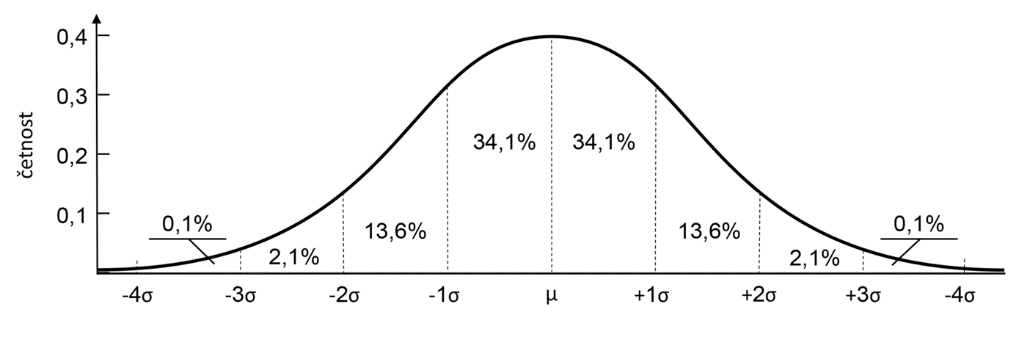
\includegraphics[width=0.9\linewidth]{gauss.png}}
\end{frame}

\begin{frame}
\frametitle{Additive Gaussian noise in Matlab}
\begin{block}{randn}
randn(sz) - returns matrix of size sz (e.g. sz = size(I)) with random elements from a normal distribution with $\sigma = 1$ a $\mu = 0$.
\end{block}

\begin{block}{Exercise}
Create a function zasum(I, sigma), which takes an image I (we can expect this to be in the double type and grayscale) and adds additive Gaussian noise with $\mu = 0$ and $\sigma = \sigma$. Make sure that the output is within the range 0 to 1. Test the function on an image with different values of $\sigma$.
\end{block}
\end{frame}

\subsection{Salt and Pepper}
\begin{frame}
\frametitle{Salt and Pepper}
\begin{block}{Salt and Pepper}
Salt and pepper noise occurs when a pixel becomes completely dark or bright. 
\end{block}

\begin{block}{rand}
rand(sz) - returns a matrix of size sz with a uniform distribution in the range from 0 to 1.
\end{block}


\begin{block}{Exercise}
Create a function okoren(I, p1, p2), which takes a grayscale image I (in double type) and adds salt and pepper noise such that with the probability of p1 we obtain a fully bright pixel and with the probability of p2 we obtain a fully dark pixel. Test the function with different parameters.
\end{block}
\end{frame}


\section{Smoothing}
\subsection{Averaging}
\begin{frame}
\frametitle{Smoothing}
\begin{block}{Why smoothing}
When a human looks at a noisy image it is still possible to process and understand it. However we will be using various techniques that are sensitive to noise. It is therefore sometimes necessary to suppress the noise. This can be achieved by smoothing the image.
\end{block}
\end{frame}

\begin{frame}
\frametitle{Convolution}
\begin{block}{Convolution - Integral version - Real Numbers}
\begin{equation*}
J= I \ast M \iff J (\chi, \psi) = \int_{-\infty}^{\infty}\int_{\infty}^{\infty} I(x,y)M(\chi - x,\psi - y) dx dy
\end{equation*}
\end{block}

\begin{block}{Convolution - Discrete version - Real Numbers}
\begin{equation*}
J = I \ast M \iff J(r,c) = \sum_{u=-\infty}^{\infty}\sum_{v=-\infty}^{\infty} I(u,v)M(r-u,c-v)
\end{equation*}
\end{block}

\end{frame}

\begin{frame}
\frametitle{Convolution}
\noindent\makebox[\textwidth]{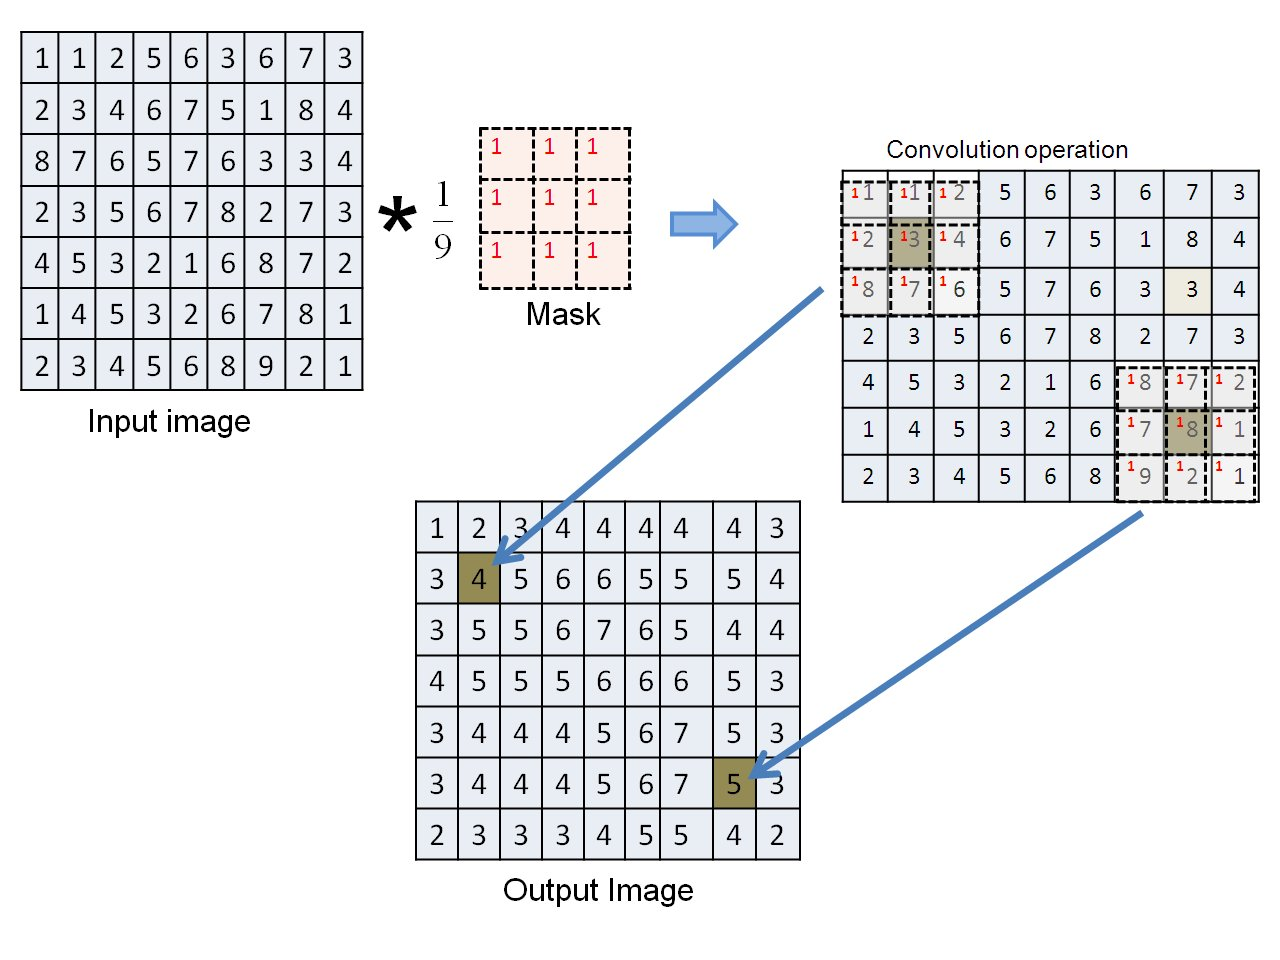
\includegraphics[width=0.9\linewidth]{convolution.jpg}}
\end{frame}

\begin{frame}
\frametitle{Convolution - Matlab}
\begin{block}{conv2}
conv2(A,B) - performs convolution of matrices A and B.
\end{block}

\begin{block}{imfilter}
imfilter(I,f) - applies a convolutional filter f on the image f
\end{block}

\begin{block}{imfilter}
imfilter(I,f, 'option') - option changes the size of the resulting image (e.g. 'same') by deciding what values are used when the convolution ''looks'' outside of the image (for example: 'replicate', 'symmetric'). It is possible to use multiple options at the same time.
\end{block}
\end{frame}

\begin{frame}
\frametitle{Convolution - filters}
\begin{block}{Manual}
Filters can be created manually e.g. averaging filter is ones(3)/9.
\end{block}

\begin{block}{fspecial}
fspecial('name', params) - returns a filters based on name and params.
\end{block}

\begin{block}{fspecial}
fspecial('average',hsize) - returns the averaging filter with size hsize \\
fspecial('gaussian',hsize,sigma) - returns a Gaussian filter
\end{block}
\end{frame}

\begin{frame}
\frametitle{Convolution filters}
\begin{block}{Exercise}
Display the Gaussian filters of various sizes and sigmas.
\end{block}

\begin{block}{imgaussfilt}
imgaussfilt(I, sigma) - filters the image with a Gaussian filter with a given sigma. This is more efficient than fspecial with imfilter.
\end{block}

\begin{block}{Exercise}
Add noise to an image with the method zasum. Try to suppress the noise with smoothing try this for the salt and pepper noise as well.
\end{block}
\end{frame}

\subsection{Median filtration}
\begin{frame}
\frametitle{Median filtration}
\begin{block}{Median filtration}
For salt and pepper noise the averaging method is not effective. A different approach is therefore necessary. Instead of averaging we will use the median value for each filtration window.
\end{block}

\begin{block}{medfilt2}
medfilt2(I, [m n]) - returns the image after median filtration with window size of m $\times$ n.
\end{block}

\begin{block}{Exercise}
Add Gaussian noise to an image and apply the median filtration. Try this also for the salt and pepper noise with various parameters.
\end{block}
\end{frame}

\section{Image sharpening}
\subsection{Unsharp Masking}

\begin{frame}
\frametitle{Unsharp masking} 
\noindent\makebox[\textwidth]{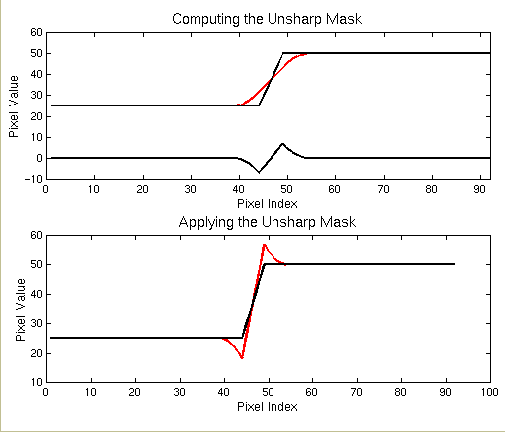
\includegraphics[width=0.9\linewidth]{unsharp.png}}
\end{frame}

\begin{frame}
\frametitle{Unsharp masking} 
  \begin{block}{Sharpening}
    We want to sharpen a blurred image. This task is similar to amplifying the edges.
  \end{block} 
 
  \begin{block}{Unsharp masking - princíp}
    $I_{sharp} = I_{original} + p \cdot \left( I_{original} - I_{smooth} \right)$
  \end{block}
  
  \begin{block}{Úloha}
  Create a function unsharp\_mask(I,p,sigma), which applies unsharp masking with the parameter p with the use of addiive Gaussian noise with the parameter sigma. Apply this on the image blurred.pgm
  \end{block}
\end{frame}
\end{document}